This section will detail the project structure employed in order to construct the application, from the modified methodology used to the projected schedule and utilized technologies.

\subsection{Methodology}
Due to the size of the group for the task at hand, it was decided that a Scrum methodology modified with group micromanagement would be used. The group was split between two camps -- three worked on the design, research and evaluation of the project, and six worked on the programming itself (see figure \vref{GroupTable}). At the top of each group was one individual responsible for managing their group's workload for the week to ensure deliverables were met, and finally collaborating everything at the end of the week into a format that was presentable to the client. As much as possible, this workload was split between smaller teams that were independent and relied as little as possible on each other in order to minimize the possibility of a domino effect in missing project deadlines.

\begin{figure}[p]
\begin{centering}
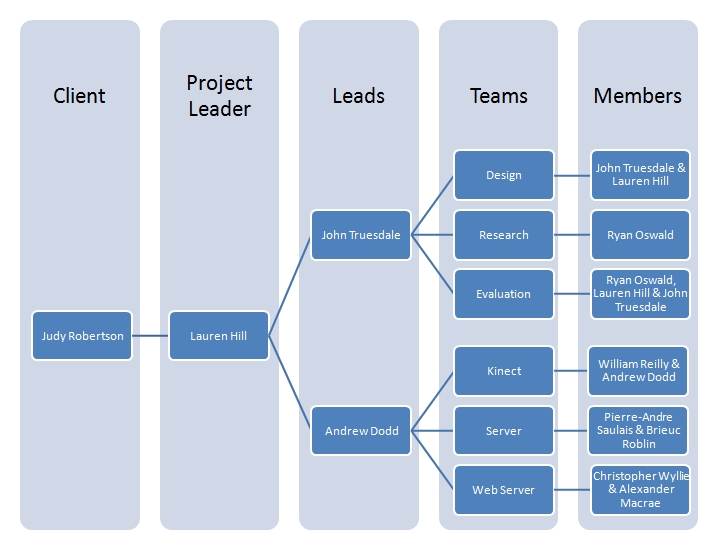
\includegraphics[width=\textwidth]{Diagrams/GroupTable.jpg}
\par\end{centering}

\caption{Group Management Table}
\label{GroupTable}
\end{figure}

\subsection{Timetable}
A routine schedule was decided for each week in order to facilitate regular meetings with the client and ensure the application's constant progression in the right direction. Each week a prototype was presented in a meeting with the client, where feedback was then received and a deliverable was decided for the week after. The group then met separately at least once a week to discuss how to achieve each deliverable with appropriate deadlines for each team, group and on an individual basis. A white board was used to document these tasks, as each member had easy access to it, and was referred to the week after for assessment of the group's progress. If needed, the group met again prior to the client's meeting or members of smaller teams met separately as needed to produce deliverables.

\subsection{Technology Utilized}
To keep the group in good contact with each other, BaseCamp was used as an online collaborative tool where announcements were made, milestones were set and each meeting's minutes were posted. This was to ensure that each member had the adequate resources and information in order to work towards their own personal deliverables. In addition GitHub was used as online source control in and was maintained solely by the code group leader\footnote{\url{https://github.com/andrewdodd13/kinect-balloons}}.

\clearpage{}

\subsection{Project Schedule}
At the start of the project, a rough outline of all high level project deliverables was laid out within the twelve week timespan. This rough draft provided the project lead with a way of correlating at which point the group was in at any given time and thus determining if the project was on track. As an agile method was used to construct the application, each week the plan was updated, for better or for worse, and was modified to meet the client's weekly deliverables. The modified draft is detailed below:

\begin{description}
	\item[Week 1] - Client Specification
	\item[Week 2] - Initial Concept
	\item[Week 3] - Paper Prototype
	\item[Week 4] - Application Iteration \textit{(2)}
	\item[Week 5] - Client Evaluation
	\item[Week 6] - Application Iteration \textit{(3)} \textbf{*}
	\item[Week 7] - Client Evaluation
	\item[Week 8] - Application Iteration \textit{(4)} and User Evaluation
	\item[Week 9] - Evaluation and Application Iteration \textit{(5)} \textbf{*}
	\item[Week 10] - Draft Report and User Evaluation
	\item[Week 11] - Report Revision, Evaluation and Application Iteration \textit{(6)}
	\item[Week 12] - Final Report
\end{description}

\textbf{*} - A number of contingency weeks were placed within the initial timetable for additional development if required. If the contingency week was not needed, the objective was to produce further functionality and provide another iteration.
